\section{Conformational Fluctuations of the Rotaxane}

% Electrophoretic, electro-osmotic and entropic forces are, in principle, acting on the
% rotaxanes. The electrophoretic force sets the negatively charged DNA in motion, under the
% action of the applied bias (from cis to trans for $Delta V > 0$). Electroosmosis
% generates an opposing force, arising from the motion of cations accumulated on the walls
% of the negatively charged ClyA pore and the DNA thread. Finally, the entropic force is
% solely geometry specific, and pushes the rotaxane towards conformations with high
% configurational entropy
%
% Entropic forces are expected to play an important role in the rotaxanes studied here,
% which are composed of stiff dsDNA and flexible ssDNA parts.
%
% Rarely the toehold is caputered inside the nanopore. Occurs more often when the applied
% voltage induces an upward force on the rotaxane. This process is important in explaining
% why the cycles are faster at positive than at negative applied potentials, but were
% slower as the potential was increased.
%

% conformational fluctuations are observed induced by the large fraction of flexible
% ssDNA.
% These fluctuations enable the cis-neutravidin bead to explore the cis-reservoir and find
% cargo strands to hybridise.
%
% Lowering the opposing bias below $-\ 70\ mV$ induces a transition in the rotaxane cycle,
% suggesting the capturing of the interface in inside of the pore. This impedes the
% hybridisation reaction since the toehold is sequestered inside of the pore.

\begin{equation}
  X = \begin{cases}
        &Z_0 + |\textbf{r} - \textbf{r}_{cis}|, \hspace{0.5cm} \textit{if on cis-side}\\
        &Z, \hspace{2.5cm} \textit{if inside pore}\\
        &-|\textbf{r}|, \hspace{2.11cm} \textit{if on trans-side}
      \end{cases}
\end{equation}


\begin{figure}
\begin{center}
  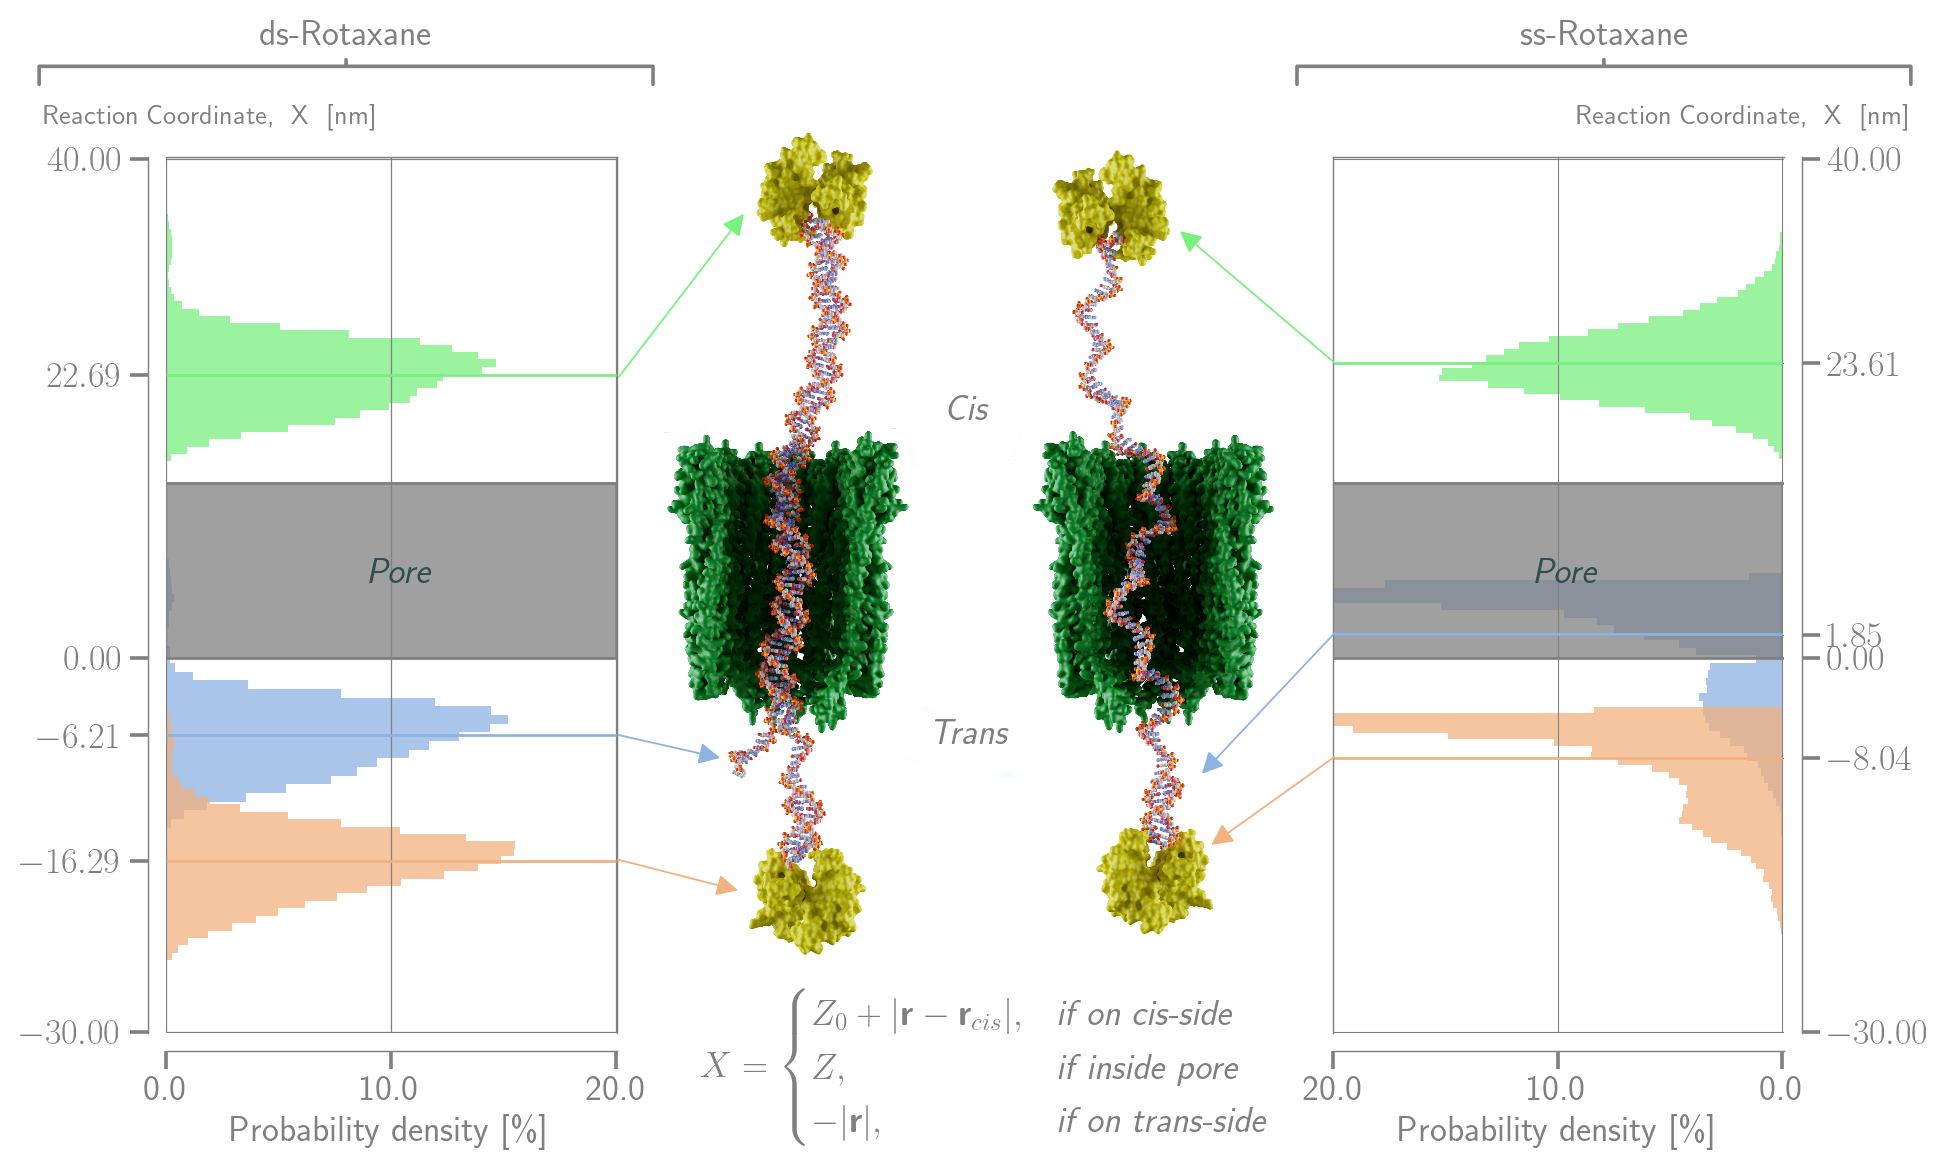
\includegraphics[width=0.90\textwidth]{Figures/RotaxaneFluctuations.png}
  \caption{write caption}
\end{center}
\end{figure}
